\spChapter[Math Environment]{Math Environment}

    \section{Math Writing Support}
        \texttt{spBook} load some essential math macro packages to support math writting, even some complex formula.
        \begin{align}
            \hspace{-25pt}\Gamma_{n\mathbf{Q}}^{\mathrm{ex-ph}}\left(T\right)&=\frac{2\pi}{\hbar}\frac{1}{\mathcal{N}_\mathbf{q}}\sum_{m\nu\mathbf{q}}\left|\mathcal{G}_{nm\nu}(\mathbf{Q},\mathbf{q})\right|^2\left[\left(N_{\nu\mathbf{q}}+1+F_{m\mathbf{Q}+\mathbf{q}}\right)\times\delta\left(E_{n\mathbf{Q}}-E^\prime_{m\mathbf{Q}+\mathbf{q}}-\hbar\omega_{\nu\mathbf{q}}\right)\right.\nonumber
            \\
            &\left.+\left(N_{\nu\mathbf{q}}-F_{m\mathbf{Q}+\mathbf{q}}\right)\times\delta\left(E_{n\mathbf{Q}}-E^\prime_{m\mathbf{Q}+\mathbf{q}}+\hbar\omega_{\nu\mathbf{q}}\right)\right]
        \end{align}

    \section{\texttt{tikz} and \texttt{tikz-cd}}
        The \texttt{spArticle} class automatically  loads the \texttt{tikz} package, allowing you to create diagrams and figures directly without any additional configuration.\footnote{This figure's origin code is copy from \href{https://www.mathcha.io/}{mathcha}.}
        \tikzset{every picture/.style={line width=0.75pt}}
        \begin{figure}[H]
            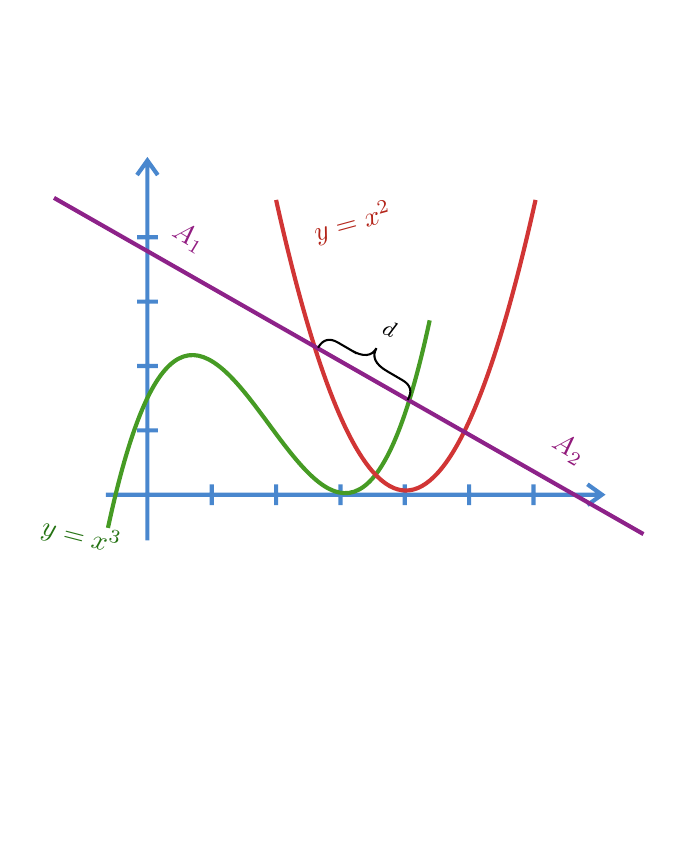
\begin{tikzpicture}[x=0.75pt,y=0.75pt,yscale=-1,xscale=1]
                \draw [color={rgb, 255:red, 73; green, 135; blue, 206 }  ,draw opacity=1 ][line width=1.5]  (246,173) -- (485,173)(266,12) -- (266,195) (478,168) -- (485,173) -- (478,178) (261,19) -- (266,12) -- (271,19) (297,168) -- (297,178)(328,168) -- (328,178)(359,168) -- (359,178)(390,168) -- (390,178)(421,168) -- (421,178)(452,168) -- (452,178)(261,142) -- (271,142)(261,111) -- (271,111)(261,80) -- (271,80)(261,49) -- (271,49) ;
                \draw   ;
                \draw  [color={rgb, 255:red, 70; green, 155; blue, 36 }  ,draw opacity=1 ][line width=1.5]  (247,189) .. controls (298.67,-51) and (350.33,329) .. (402,89) ; 
                \draw  [color={rgb, 255:red, 209; green, 53; blue, 53 }  ,draw opacity=1 ][line width=1.5]  (328,31) .. controls (369.67,217.67) and (411.33,217.67) .. (453,31) ;
                \draw [color={rgb, 255:red, 141; green, 34; blue, 137 }  ,draw opacity=1 ][line width=1.5]    (221,30) -- (505,192) ;
                \draw  [line width=0.75]  (391.4,127.4) .. controls (393.75,123.37) and (392.91,120.18) .. (388.88,117.83) -- (381.48,113.51) .. controls (375.72,110.15) and (374.02,106.45) .. (376.37,102.42) .. controls (374.02,106.45) and (369.96,106.79) .. (364.21,103.43)(366.8,104.94) -- (357.78,99.68) .. controls (353.75,97.33) and (350.55,98.17) .. (348.2,102.2) ;
                \draw (286,49) node  [color={rgb, 255:red, 146; green, 29; blue, 130 }  ,opacity=1 ,rotate=-30.96]  {$A_{1}$};
                \draw (469,151) node  [color={rgb, 255:red, 145; green, 25; blue, 123 }  ,opacity=1 ,rotate=-30.96]  {$A_{2}$};
                \draw (234,193) node  [color={rgb, 255:red, 36; green, 114; blue, 18 }  ,opacity=1 ,rotate=-14.47]  {$y=x^{3}$};
                \draw (365,42) node  [color={rgb, 255:red, 179; green, 35; blue, 24 }  ,opacity=1 ,rotate=-344.74]  {$y=x^{2}$};
                \draw (382.8,93.2) node  [font=\footnotesize,rotate=-22.93]  {$d$};
            \end{tikzpicture}
            \vspace{-80pt}
            \caption{tikz draw graph example}
        \end{figure}
        \begin{figure}[H]
            \centering
            \begin{tikzcd}
                T
                \arrow[drr, bend left, "x"]
                \arrow[ddr, bend right, "y"]
                \arrow[dr, dotted, "{(x,y)}" description] & & \\
                & X \times_Z Y \arrow[r, "p"] \arrow[d, "q"]
                & X \arrow[d, "f"] \\
                & Y \arrow[r, "g"]
                & Z
            \end{tikzcd}
            \caption{commutative diagram demo1}
        \end{figure}
        \begin{figure}[H]
            \begin{tikzcd}[row sep=scriptsize, column sep=scriptsize]
                & f^* E_V \arrow[dl] \arrow[rr] \arrow[dd] & & E_V \arrow[dl] \arrow[dd] \\
                f^* E \arrow[rr, crossing over] \arrow[dd] & & E \\
                & U \arrow[dl] \arrow[rr] & & V \arrow[dl] \\
                M \arrow[rr] & & N \arrow[from=uu, crossing over]\\
            \end{tikzcd}
            \caption{commutative diagram demo2}
        \end{figure}

    \section{Math Statement Index}
        \texttt{spBook} has set a function that 
        \begin{definition}
            A \emph{monoid} is a set with an associative binary operation and an identity element.
        \end{definition}
        \begin{lemma}[Schur Lemma]
            A \emph{monoid} is a set with an associative binary operation and an identity element.
        \end{lemma}
        \begin{theorem}[Schur Theorem]
            A \emph{monoid} is a set with an associative binary operation and an identity element.
        \end{theorem}